% !TEX root = ../main.tex
\section{Variation across evaluation seeds}
\label{app:seedvariability}

Table~\ref{tab:headlineseedsd} reports standard deviations across independent sampling seeds for all our settings in Tables~\ref{tab:headlinecomparison} and~\ref{tab:headlinelownfe}, together with the SCCFG 2 MATH500 settings used in Figure~\ref{fig:headlinestages}. Each seed generates one solution per problem across the full fixed test set. For seed accuracies $a_1,\ldots,a_n$, expressed as percentages, we report the mean $\bar a$ and sample standard deviation
\[
  s_a=\sqrt{\frac{1}{n-1}\sum_{r=1}^{n}(a_r-\bar a)^2}.
\]
These values describe generation randomness at a fixed checkpoint and test set. They are distinct from uncertainty across test problems and from variation across training runs. We use every completed sampling seed at each denoising budget: $n=64,32,16,8$ for NFE $8,16,32,64$, respectively. Checkpoints, guidance, scorers, and benchmark populations match the main tables.

% !TEX root = ../main.tex
\begin{table}[htbp]
\caption{Mean accuracy $\pm$ standard deviation across sampling seeds, in percentage points. Each seed evaluates the complete benchmark at the same fixed checkpoint. Columns use 64, 32, 16, and 8 seeds, respectively. The 64-NFE column supplies the results in Table~\ref{tab:headlinecomparison}; SCCFG 3 supplies the MATH500 rows in Tables~\ref{tab:headlinecomparison} and~\ref{tab:headlinelownfe}. SCCFG 2 MATH500 rows correspond to Figure~\ref{fig:headlinestages}.}
\label{tab:headlineseedsd}
\centering\small
\setlength{\tabcolsep}{4pt}
\begin{tabular}{@{}lrrrr@{}}
\toprule
Model / stage & 8 NFE & 16 NFE & 32 NFE & 64 NFE\\
\midrule
\multicolumn{5}{@{}l}{\textit{GSM8K, ELF-B, SCCFG 2}}\\
Pre-NFT & $26.40\pm0.87$ & $34.48\pm0.94$ & $37.80\pm1.20$ & $39.17\pm0.63$\\
Post-NFT & $30.08\pm0.87$ & $37.77\pm0.84$ & $41.13\pm0.94$ & $42.16\pm0.88$\\
\addlinespace
\multicolumn{5}{@{}l}{\textit{GSM8K, ELF-L, SCCFG 2}}\\
Pre-NFT & $49.41\pm0.86$ & $55.33\pm0.91$ & $57.88\pm1.03$ & $58.67\pm0.69$\\
Post-NFT & $54.84\pm0.92$ & $60.55\pm0.69$ & $62.47\pm0.82$ & $63.74\pm0.83$\\
\addlinespace
\multicolumn{5}{@{}l}{\textit{MATH500, ELF-L, SCCFG 3}}\\
Pre-NFT & $15.23\pm1.16$ & $17.93\pm1.30$ & $19.65\pm1.37$ & $21.18\pm0.70$\\
Post-NFT & $17.45\pm1.33$ & $20.93\pm1.26$ & $22.60\pm1.58$ & $24.68\pm1.27$\\
\addlinespace
\multicolumn{5}{@{}l}{\textit{MATH500, ELF-L, SCCFG 2}}\\
Pre-NFT & $13.88\pm1.19$ & $16.39\pm1.20$ & $17.89\pm1.31$ & $18.85\pm1.38$\\
Post-NFT & $16.31\pm1.36$ & $20.09\pm1.23$ & $22.08\pm1.41$ & $23.60\pm1.79$\\
\addlinespace
\bottomrule
\end{tabular}
\end{table}


\section{ELF-B inference allocation before and after NFT}
\label{app:elfbbudgets}

Figure~\ref{fig:elfbstages} complements the ELF-L comparison in Figure~\ref{fig:headlinestages}. It uses the GSM8K supervised epoch-18 and NFT-update-300 checkpoints with async $(2.5,2,1.5)$ and SCCFG 2. Y-axis ranges are matched across training stages separately for oracle accuracy and voting.

\begin{figure}[htbp]
\centering
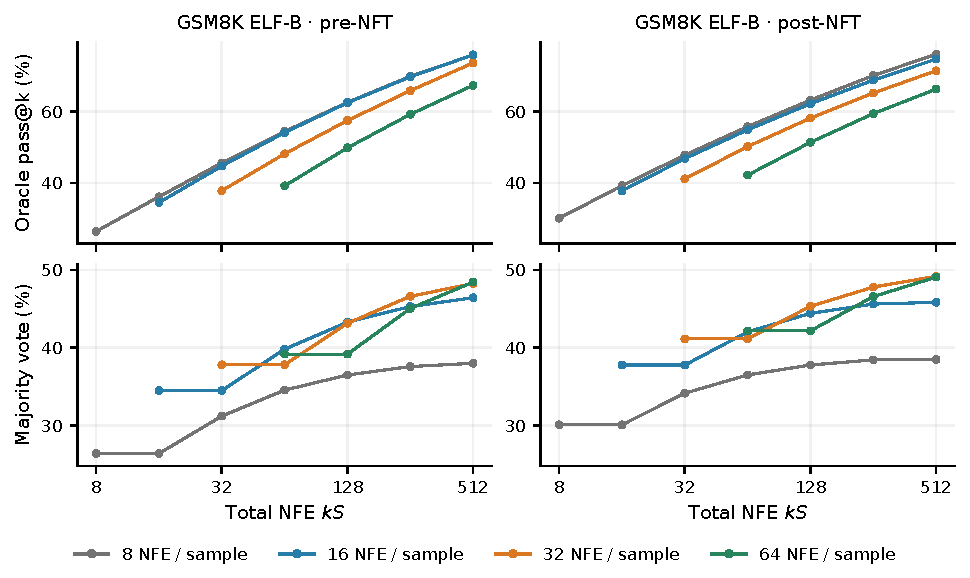
\includegraphics[width=\linewidth]{figures/appendix_elf_b_stages_sccfg2.pdf}
\caption{GSM8K ELF-B before and after NFT. Upper panels show oracle pass@$k$; lower panels show majority-vote accuracy. Colors denote denoising NFE per sample. The same 64/32/16/8 sample cohorts and total budget of 512 denoising calls are used as in Figure~\ref{fig:headlinestages}.}
\label{fig:elfbstages}
\end{figure}
